\section{Design and Implementation}
\label{sec:implement}

\NM{} is designed as a drop-in replacement for the default memory allocator. It intercepts all memory allocation/deallocation APIs via the preloading mechanism. 

For its memory management, \NA{} utilize some known mechanisms of existing allocators. First, it utilizes the size class to manage objects. Instead of allocating the exact size, \NA{} will round the size of an allocation to its closest size class. Similar to TcMalloc~\cite{tcmalloc}, \NA{} also utilizes fine-grained size classes for small objects, such as 16 bytes apart for objects less than 128 bytes, and 32 bytes apart for objects between 128 bytes and 256 bytes, then power-of-2 afterwards. Second, it utilizes the ``\textbf{Bi}g-\textbf{B}ag-\textbf{o}f-\textbf{P}ages'' mechanism to manage objects, and separates the metadata from actual objects. Since all objects in the same page will have the same size class, \NA{} only tracks the size information for one page, which helps reduce the memory overhead for metadata. Third, \NA{} also utilizes a size-class based freelist to manage freed objects. Every freed object will be added into a corresponding freelist, and objects in the freelist will be allocated first in order to reduce possible cache misses. Further, \NA{} utilizes the first word of freed objects to link different objects, which is similar to Linux and TcMalloc~\cite{tcmalloc}. This mechanism helps to reduce memory overhead, but is prone to memory vulnerabilities, such as buffer overflows and double-frees~\cite{Guarder}.     


Different from existing work, \NA{} aims to reduce remote accesses, and balance the workload between different hardware nodes. It also utilizes huge page support to improve the performance, and designs its interleaved and blockwise memory allocation to accommodate shared objects. It includes multiple components as discussed in the following. 

\begin{figure*}[h]
\begin{center}
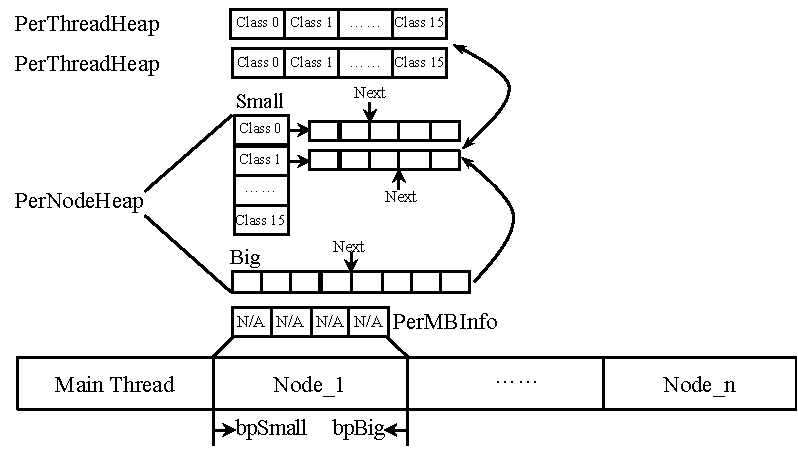
\includegraphics[width=0.8\textwidth]{figure/heaplayout}
%\includegraphics{figure/overview2}
\end{center}
\vspace{-0.1in}
\caption{Overview of \NA{}.
\label{fig:overview}}
\vspace{-0.1in}
\end{figure*}

\subsection{Topology Aware Task Assignment} 
\label{sec:taskassign}

Due to the importance of task assignment to  memory locality, \NA{} designs a topology-aware task assignment, which builds the basis for its memory management. In general, every thread will be bound to a specific node so that all memory allocations will be satisfied from the node locally, as described in Section~\ref{sec:nodeaware-memory}. However, \NA{} manages memory from the initial thread differently, as described in Section~\ref{sec:mainthread}. 

During the initialization phase, \NA{} recognizes the relationship between each CPU core and each memory node. It further intercepts all thread creations in order to bind a newly-created thread to a specific node. Note that a thread is pinned to a node, instead of a core, which still allows the OS scheduler to perform the load balance when necessarily.

In order to balance the workload among multiple nodes, \NA{} takes a round-robin manner to assign tasks, which is similar to TBB-NUMA~\cite{Majo:2015:LPC:2688500.2688509}.  This ensures that each processor will have a similar number of threads, and therefore a similar workload. This balance also prevents the node imbalance issue of the memory as described in Section~\ref{sec:numa}. To bind a thread to a specific node, \NA{} employs \texttt{pthread\_attr\_setaffinity\_np} to set the attributes of a thread, and passes the attribute to its thread creation function. 

\subsection{Node-Aware Memory Management} 
\label{sec:nodeaware-memory}

\NA{} utilizes multiple existing mechanisms to ensure the node-aware memory management. First, it specifies the physical NUMA node explicitly for a block of virtual memory with the NUMA API (e.g., \texttt{mbind}), when a block of memory is allocated from the OS. This is the same  as  previous work~\cite{tcmallocnew}. Second, \NA{} maintains per-node freelists and per-thread freelists to track freed objects, and handles large objects and small objects differently. The assumption is that an application typically has a large number of small objects, but with relatively fewer big objects.  More specifically, freed objects with the size larger than 512KB will be always tracked in the per-node freelist, while \NA{} maintains per-node freelist and per-thread freelist for small objects.  During the memory deallocation, \NA{} will determine the physical address and the size information of an object in order to place it correspondingly. A large object is always placed into a per-node freelist, while the placement of a small object will be based on its location information: if the object is allocated from a different node, it will be placed into the common freelist of that node; Otherwise, it will be placed into the per-thread freelist. Freed objects will be used to satisfy  allocation requests before never-allocated objects, in order to reduce  memory consumption and reduce possible cache misses.  
%Third, during the allocation, \NA{} will be always satisfied by objects in the freelist first. 

Different from existing work, \NA{} reduces the overhead of frequent system calls, and designs a mechanism that could quickly locate the size information. The basic idea can be seen in Figure~\ref{fig:overview}. Basically, \NA{} utilizes the huge address space of 64-bits machine. Instead of frequently allocating the memory from the OS, \NA{} obtains a big chunk of memory from the underlying OS initially, and then divides it to multiple chunks with the same size. Each chunk will be bound to a specific memory node with the NUMA API support, as described in the above. Therefore, the physical node information could be obtained from the virtual address directly, by checking the distance from the starting address of the heap. Then a freed object will be always returned to its original node, either on the per-node freelist or the per-thread freelist of the current thread. During the allocation, the request will be always satisfied from the freed lists that always keeps freed objects in the local node, or from never-used objects that are allocated from the local node (via NUMA API). Therefore, \NA{} guarantees local allocations that the physical pages are originated from the current node that the current thread is running on, since a thread never changes its node during the whole execution. Such a mechanism ensures the good locality for private objects, but not good for objects that are shared by multiple threads. 

 %The information will be utilized to determine where to place a freed object.  \NA{} utilizes per-node freelis
%Since every thread is already pinned to a specific node, its allocations could only be satisfied from  its local node. \NA{} designs the per-node heap to hold objects that were allocated by a local thread but deallocated by a remote thread. If an object is deallocated by a local thread, it will be placed into the per-thread heap of the current thread. \NA{} eliminates the usage of locks for such deallocations.      

\subsection{Interleaved and Blockwise Memory Allocation for Shared Objects} 
\label{sec:mainthread}

Based on our observation, most NUMA performances issues identified by existing NUMA profilers are related to shared objects~\cite{XULIU, MemProf}. These shared objects are typically allocated in the main thread, but were accessed concurrently by multiple children threads. For existing allocators, these shared objects were allocated locally in the node where the main thread is running on, due to the first-touch policy of physical memory. \NA{} proposes to identify shared objects with the allocation/deallocation pattern, and then infers the OS to allocate physical memory in an interleaved and blockwise way. Basically, shared objects will be allocated from a block of memory that its page allocations will be interleaved across all physical nodes, which will reduce the load imbalance problem. \NA{} further proposes to allocate the physical memory in a blockwise way if an allocation is involved with multiple physical pages, as shown in Figure~\ref{}.   
 
% However, this policy may cause multiple performance issues. First, it may cause load imbalance issue where the initial node have much more accesses than other nodes. Second, it may lead to a large number of remote accesses, since children threads may not run in the same node as the main thread. To address such issues, \NA{} proposes to identify shared objects with the allocation/deallocation pattern, and then infers the OS to allocate physical memory in an interleaved and blockwise way. \NA{} assumes that objects from the same allocation site will have a similar pattern, since that depends on the program logic. If a newly-allocated object has been deallocated in the main thread before creating children threads, then this object cannot be shared by multiple threads. Therefore,  \NA{} monitors the allocation and deallocation pattern for heap objects. If a calllsite is considered to have shared objects, 
  
%If an object is not shared between multiple threads, most existing allocators will allocate such objects from the local node, causing no performance issue.   the main thread typically prepares the data for all of its children threads. That is, it is very likely that most objects allocated from the main thread will be shared by most threads. Therefore, it will cause the load imbalance issue, if all objects from the main thread are allocated from the node that the main thread is running on. Also, it could also introduce significant number of remote accesses, since not all threads could run on the same node.  

%\paragraph{Children Threads:} For normal threads, it is better to allocate the memory from the local node, in order to reduce remote accesses. But existing allocators have an issue to handle remote frees that the deallocation thread is not the same as the allocation thread~\cite{Aigner:2015:FML:2814270.2814294}. They tend to place freed objects into the current thread, such as TCMalloc~\cite{tcmalloc} or jemalloc~\cite{jemalloc}, no matter where these objects are allocated from.  However, this could cause remote accesses. In order to solve this issue, \NM{} proposes an information-computable design, as shown in Figure~\ref{fig:overview}. Basically, \NM{} utilizes the fact of 64-bit address space, where machines have extremely large amount of virtual address. Basically, \NM{} requests 32 TB virtual address at one time, and then divides it to multiple spans based on the number of nodes. For each span, \NM{} binds the memory to a specific node through \texttt{mbind} system call. Therefore, \NM{} is able to recognize the physical location by the address. During the deallocation, \NM{} will actually return a remote object to its owner, and only return the objects from the current node to the current thread's PerThreadHeap. 


\paragraph{Automatic Huge Page Support:} The default huge page support is not good for the performance~\cite{}. It also may have some harmful impact on the performance. However, if the huge page is utilized very well, the application's performance can be improved dramatically. The underlying reason is that it will lead to less TLB misses, since one TLB entry will cover a larger range of memory, such as 2MB instead of 4KB. Based on a simple test, using the TLB could improve a simple test case more than 10\%, without any other changes. To taking advantage of this benefit, each PerNodeHeap is further divided into two parts, where small objects will be allocated from the beginning and will be allocated using small pages, while big objects will be allocated from the end of the heap using huge page (2MB). We believe that this mechanism balances the performance and memory consumption.   

\paragraph{Reutilization of Big Objects:} Existing allocators will handle big objects different with small objects, which will be allocated from the OS directly. When these objects are freed, they will be returned to the OS directly by invoking \texttt{munmap} or \texttt{madvise}. This mechanism was designed to reduce memory consumption. However, this mechanism will invoke a lot of unnecessary overhead, since a big object may include numerous pages and cache lines.  Returning big objects to the OS may require to reload these pages and cache lines if an application actually requires more memory.  
%Taking an object with the size of 1 MB as the example, this object includes 256 pages (4KB). Therefore, the overhead includes returning 256 pages to the OS (by modifying the page table entries of 256 pages), and then 256 page faults when this is returned. 
%More importantly, cache lines of these 256 pages should be reloaded from the memory after allocating these physical pages. 
%\NM{} aims to reduce such overhead based on a simple assumption: if the application is requesting memory, then big objects should not be returned to the OS to avoid such overhead. In fact, 
\NM{} proposes to utilize these big objects for small objects, instead of returning them back to the OS. Due to this design, \NM{} actually utilizes 1MB as the basic unit, and then allocates 1MB for small objects on demand. 

\paragraph{Node-local Metadata:} \NM{} designs the metadata meticulously, which will be always allocated in the same node. Such metadata includes the PerMBInfo, freelists for different size classes, and freelists for big objects. PerThreadHeap's metadata will be also allocated in the local node as well, which has been assigned to a specific node during thread creation. 


\subsection{Node-Local Allocation}

What is the basic idea of allocation? 
Basically, upon receiving a request, \NM{} will check the size of the object at first. If the size is less than the threshold of big objects, this is a small object. 

For small objects, \NM{} will always allocate them from the PerThreadHeap. Since a PerThreadHeap will be only utilized by one thread, it won't need the synchronization, and possibly has the better scalability. 

\subsection{Special Support for Main Thread}
\NM{} provides the special support for the main thread, which is motivated by a lot of existing tools ~\cite{XULIU, MemProf}. Based on their paper, many of NUMA related performance problems are caused by one type of objects that were allocated in the main thread but shared by multiple children threads. To prevent these issues, they proposed to change the code explicitly, using a group of threads that were bound to different nodes to perform the initialization. However, these changes are not automated, which should also rely on the test results of these NUMA tools.  

Instead, \NM{} proposes an automatic method to deal with these issues. Due to the fact that many objects will be shared by children threads later, \NM{} allocates objects from the main thread in a separate heap, which mainly focuses on the load imbalance. To achieve the load balance, one simple technique is to allocate objects that will be physically allocated with an interleaved way. However, this simple technique does not work due to the following reasons. 

First, not all objects are shared by multiple threads. Some objects will be just accessed by the main thread. For these objects, if their corresponding physical pages are allocated in remote nodes, they could  incur remote accesses unnecessarily. Therefore, \NM{} should avoid unnecessary remote accesses by recognizing which objects are private objects, and allocating these objects locally.  

Second, load balance alone cannot guarantee the optimal performance, if objects are accessed block-wise by multiple threads. In fact, this is more common based on existing studies~\cite{XULIU, MemProf}. \NM{} supports block-wise memory allocation for big objects.  

Third, the allocation should take advantage of huge pages that is already available in most existing hardware. \NM{} takes this into account for its design and implementation. In fact, \NM{} divides the memory into three spans. 

Fourth, big objects will utilize a lot of memory, which should be handled carefully. We can't reutilize these objects for node-local allocations, which may incur unnecessary remote accesses. Also, we don't want to waste the physical memory for these objects. Instead, \NM{}  will return these objects to the OS directly during the deallocation. 

During the implementation, \NM{} should detect private objects. It utilizes a simple rule to detect private objects: if an object is deallocated in the main thread before the creation of children threads, then this object is not shared by other threads. However, if an object has been allocated in the special heap, it cannot be changed easily with a low overhead. We further propose a call-site based mechanism: objects from the same callsite will typically have the same deallocation behavior. Objects will be allocated in the special heap at first, but will be allocated in the normal heap if some objects from the call callsite were identified as private objects. \NM{} therefore maintains two hashmap to track such objects: one hashmap is used to track private callsite, and another hashmap is used to track the relationship between objects and their corresponding callsites. 
During the allocation, \NM{} will check whether the callsite is private or not. If the corresponding callsite has been identified as the shared one, then it will be allocated from the special heap. If the corresponding callsite has not been tracked before, then this object will be allocated form the special heap, and the corresponding object will be placed in the hashmap that tracks the relationship between objects and their corresponding callsites. 

During the deallocation, \NM{} will check the callsite in the hashmap as well. 

For private objects, its deallocation phase is the same as the allocation phase. Therefore, we will track the phase information there. 
We will use the phase 0 to indicate that the phase is not in the main thread phase. Otherwise, we will use the number to indicate it.   

\subsection{Huge Page Support}

Modern hardware typically installs with huge page support. Huge page is a special page that its page size is much larger than 4 kilobytes. Currently, the Linux system has two page sizes, 4 Kilobytes and 2 Megabytes.  
Based on the existing study~\cite{hugepages}, huge page will be beneficial to the performance by reducing Translation Look-aside Buffer (TLB) misses.  Currently, modern OS typically employs multi-level page table design, in order to reduce physical pages used for the page table and avoid using the continuous physical pages for the page table. Due to the wide range of virtual address, now Linux employs four level page table design. However, this also indicates the huge performance lost due to the TLB misses. If a mapping cannot be satisfied in the TLB buffer, the OS will be forced to load four page table entries to perform the address translation. The loading of page table entries, typically into the data cache, could also significantly pollute the data cache. 
 
Huge page could reduce the TLB misses, and further reduce the cache pollution caused by TLB misses. However, 
However, it is 



